\chapter{Approach}
\todo{Why are we using a data-driven / machine learning approach? Show that it is complicated to do it by hand. Also write why not to do auto-tuning.}

\begin{figure}
    \centering
    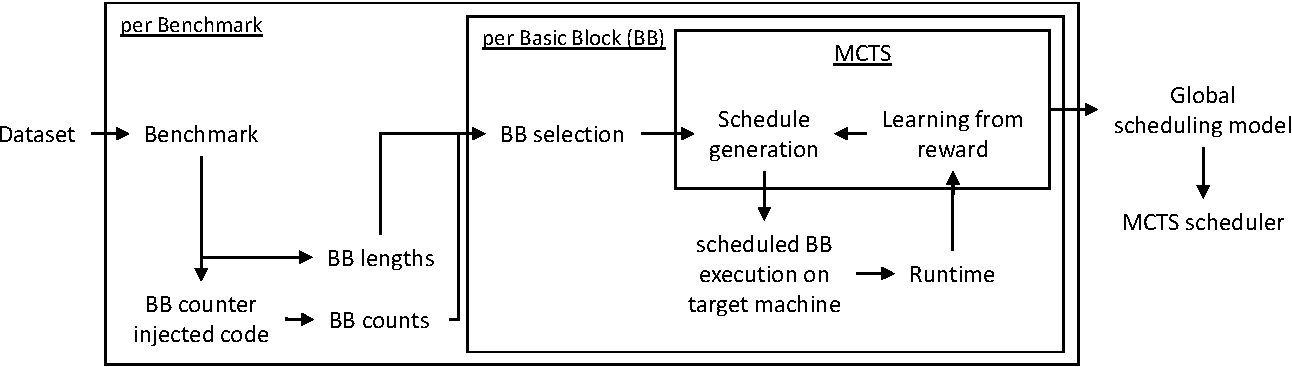
\includegraphics[width=\textwidth]{img/ppt/approach_overview-crop.pdf}
    \caption[Overview of the approach]{Overview of the overall approach. 
    The process covers the selection of basic blocks, the instruction schedule generation, the execution model, the learning process and the derivation of the final scheduler.}
    \label{fig:approach:overview}
\end{figure}

\section{Dataset}
\label{sec:approach:dataset}
\begin{enumerate}
    \item 
    \begin{itemize}
        \item What: LLVM test suite
        \item Why: free and ready to use collection of many benchmarks and test programs
        \item How: describe the dataset, add list of benchmarks?, how many benchmarks, how many basic blocks
    \end{itemize}
    \item
    \begin{itemize}
        \item What: Custom compilation process
        \item Why: More control about the compilation process is required. Insertion of optimizer passes, selection of custom schedulers
        \item How: Extract compilation arguments and execution arguments (flags, files to be read) from test suite
    \end{itemize}
\end{enumerate}
    
\section{Basic Block --- scheduling unit}
\label{sec:approach:basicblock}
\begin{itemize}
    \item What: We choose basic blocks as the scheduling unit
    \item Why: Used by the LLVM compiler framework and most other compilers, Limits scope and complexity
    \item How: Code split into BB's and scheduling of BB's independently
\end{itemize}

\subsection{Selection process}
\begin{itemize}
    \item What: Select BB's for our dataset
    \item Why: Too many to work on all of them, time intensive, compilation time, execution time, ML
    \item How: Develop heuristics for the selection
\end{itemize}
\subsubsection{Longest basic blocks}
\begin{itemize}
    \item What: The BB's with the most instructions in them
    \item Why: Good heuristic for number of scheduling decisions. From many scheduling decisions we can learn more. Short BBs have very few scheduling decisions
    \item How: Count the number of instructions in the intermediate LLVM IR files of that basic block
\end{itemize}
\subsubsection{Most executed basic blocks}
\begin{itemize}
    \item What: The BB's that are executed the most often
    \item Why: Most important blocks. Good decisions here can lead to higher speedup
    \item How: Implement LLVM optimizer pass to inject counters into each BB. Execute to count. Generate List of counts
\end{itemize}
\todo{Show example numbers}
\subsubsection{Most executed and longest basic blocks}
\begin{itemize}
    \item What: Combine the two previous heuristics
    \item Why: Most executed, can still be very short BB's. Like initilization of for loops
    \item How: Multiply both numbers
\end{itemize}
\todo{Show example}

\section{Learning to schedule}
\subsection{Local MCTS model}
\label{subsec:approach:ml:mcts}
\subsection{Global model}
\label{subsec:approach:ml:global}

\section{Data generation}
\begin{enumerate}
    \item 
    \begin{itemize}
        \item What: Need to generate data from which we can learn
        \item Why: Dataset has only the code, we need som metric to learn from
        \item How: Execute the code and measure the metric
    \end{itemize}
    \item
    \begin{itemize}
        \item What: We choose to optimize for the runtime
        \item Why: That's what users in the most situations are interested in
        \item How: Execute the BB and measure the runtime
    \end{itemize}
\end{enumerate}

\subsection{Runtime measurement unit}
It would be optimal to just measure the the scheduled instructions with perfect precision and reliability.
\subsubsection{Basic Block}
\begin{itemize}
    \item What: Measuring the basic block itself is complicated
    \item Why: we need very precise time measurements
    \item How: the typical length of a basic block ranges from a hand full of instructions to a few dozens
    \todo{Plot basic block length distribution}
\end{itemize}
\subsubsection{Function}
A specific basic block of a function might be executed multiple times during function execution.
In this situation, this is relevant in to different aspects.

% \begin{itemize}
%     \item What: Advantage: BB is executed multiple times, so its runtime is easier to measure
%     \item Why: 
%     \item How: 
% \end{itemize}
We are more interested in speedups, rather than precise execution times.


\begin{itemize}
    \item What: Measure the function which contains the basic block is bad in general
    \item Why: Different paths could be taken throught the function, e.g. if-else, loops
    \item How: 
\end{itemize}
\begin{itemize}
    \item What: In this case it is okay
    \item Why: the benchmarks are deterministic, each path is taken the same number of times between executions
    \item How: 
\end{itemize}
\subsubsection{Program}
\begin{itemize}
    \item What: Measure the execution time of the whole program
    \item Why: Easy, but unreliable because of IO operations and other noise (e.g. OS), we are only interested in a small fraction of the code
    \item How: 
    \todo{Show visualization}
\end{itemize}

\subsection{Runtime measurement methods}
\todo{Could add little experiment where we compare hardware timers vs OS access}
\subsubsection{Profiling}
\begin{itemize}
    \item What: Profilers are a bad choice for measuring precise runtimes
    \item Why: They are just not designed for it, they serve other purposes.
        Profilers are making snapshots of the running system to measure performance. 
        There is no measurement from point A to point B which leads to inaccuracies
    \item How: Read e.g. the paper of gperf \cite{graham1982gprof}
\end{itemize}
\subsubsection{Operating system methods}
% In linux(C): clock_gettime().
% Windows: QueryPerformanceCounter().
% C++: std::high_resolution_clock().
These might return different clocks depending on the used hardware.
Returns the time from the hardware the OS runs on.
Has overhead but also handles problems.
Typically best for measurements in microseconds range and longer.
\subsubsection{Hardware performance counters}
Accessed by assembly instructions.
% x86: 'rdtsc' Saves current value into EDX:EAX registers
% ARM32: mrc p15m, 0, \%0, c15, c12, 1
% AARCH64: mrs \%0, PMCCNTR_EL0
% Aurora: fencei; smir \%0, \%usrcc
Measurements in CPU cycles.
Lowest overhead available.
Access might be protected (Linux module required).
\subsection{Basic block isolation}
\subsubsection{Basic block extraction}
How to get the assembly (compilation process).
Problems: function calls (remove), jumps(only in last instr, remove), load/access (memory access, readress to stack variable)
\todo{Create table with removed instructions}
\subsubsection{Isolated basic block execution}
From extracted basic block create inline assembly with stack variable. Now executable from C/C++.
Warmup 100 runs. Timings 1000 runs. 
\subsection{Computing rewards from runtimes}
There are some outliers in the runtimes. Sort runtimes, cutoff lower and upper 5\% of the runtimes to remove outliers and compute avg of the rest.
What could be reasons for outliers?
Show some distributions of measurements to justify why we are throwing away data.

\section{Application of the learned model}
\label{sec:approach:ml-scheduler}

% Probably wrong place here, but compare approach with auto-tuning approach.
% Why not use auto-tuning? Search space size, and lack of generalization could be a reason

% \section{Breaking down the problem (maybe just chapter introduction)}
% \begin{itemize}
%     \item Schedulers run on basic blocks -> Select the most executed (hottest) BB's
% \end{itemize}

% \section{Experimentation Pipeline}
% Explain and illustrate the pipeline incl. injection of timers and counters

% \section{Benchmarking}
% \begin{itemize}
%     \item Benchmarking methods: Instrumentation, sampling -> only instrumentation makes sense here. Justify this with instrumentation vs. sampling results (our timing vs. perf timing)
%     \item Where to inject timer in BB DAG
%     \begin{itemize}
%         \item We only want to measure optimized code, but not too kleinteilig because of lacking accuracy. Problematic code is IO code
%         \item Time whole function?
%         \item Time only relevant BB's with surrounding ones (e.g., loop headers) -> Where exactly place the the timer
%         \item Provide data and examples to demonstrate decision making
%     \end{itemize} 
% \end{itemize}
% \subsection{Implementation}
% Injection of the \lstinline[language=C++]{std::chrono::high_resolution_clock}

% \section{Training setup}
% Compile with default scheduler and measure its runtime.
% Compile with our scheduler, execute the program, measure the runtime and use it to train the agent.

% \section{MCTS}
% \subsection{Tree Modeling}
% We probably want to model the interdependence between instructions. 
% But depending on the benchmark programs, only a small fraction of possible edges between instructions are available.

% \eg When in the benchmark a MOV was scheduled and after that, there are only SUB and ADD.
% We cannot schedule another MOV even though that might be the optimal schedule.

% This problem must be addressed somehow.
% There are different possibilities:
% \begin{itemize}
%     \item Declare all the states with their possible successors to different states.
%     The problem with this approach is that the number of states gets very high and most states are visited rarely, possibly only in the given benchmark/basic-block.
%     \item Probablistic Policy like in RL. (Does that exist for MCTS?)
%     This might solve the problem with unavailable edges, but it does not help with learning at all because the agent would have to learn which instructions are available, too.
%     Which is not what we want.
% \end{itemize}